\documentclass[hidelinks,12pt]{article}
\usepackage[left=0.25cm,top=1cm,right=0.25cm,bottom=1cm]{geometry}
%\usepackage[landscape]{geometry}
\textwidth = 20cm
\hoffset = -1cm
\usepackage[utf8]{inputenc}
\usepackage[spanish,es-tabla]{babel}
\usepackage[autostyle,spanish=mexican]{csquotes}
\usepackage[tbtags]{amsmath}
\usepackage{nccmath}
\usepackage{amsthm}
\usepackage{amssymb}
\usepackage{mathrsfs}
\usepackage{graphicx}
\usepackage{subfig}
\usepackage{standalone}
\usepackage[outdir=./Imagenes/]{epstopdf}
\usepackage{siunitx}
\usepackage{physics}
\usepackage{color}
\usepackage{float}
\usepackage{hyperref}
\usepackage{multicol}
%\usepackage{milista}
\usepackage{anyfontsize}
\usepackage{anysize}
%\usepackage{enumerate}
\usepackage[shortlabels]{enumitem}
\usepackage{capt-of}
\usepackage{bm}
\usepackage{relsize}
\usepackage{placeins}
\usepackage{empheq}
\usepackage{cancel}
\usepackage{wrapfig}
\usepackage[flushleft]{threeparttable}
\usepackage{makecell}
\usepackage{fancyhdr}
\usepackage{tikz}
\usepackage{bigints}
\usepackage{scalerel}
\usepackage{pgfplots}
\usepackage{pdflscape}
\pgfplotsset{compat=1.16}
\spanishdecimal{.}
\renewcommand{\baselinestretch}{1.5} 
\renewcommand\labelenumii{\theenumi.{\arabic{enumii}})}
\newcommand{\ptilde}[1]{\ensuremath{{#1}^{\prime}}}
\newcommand{\stilde}[1]{\ensuremath{{#1}^{\prime \prime}}}
\newcommand{\ttilde}[1]{\ensuremath{{#1}^{\prime \prime \prime}}}
\newcommand{\ntilde}[2]{\ensuremath{{#1}^{(#2)}}}

\newtheorem{defi}{{\it Definición}}[section]
\newtheorem{teo}{{\it Teorema}}[section]
\newtheorem{ejemplo}{{\it Ejemplo}}[section]
\newtheorem{propiedad}{{\it Propiedad}}[section]
\newtheorem{lema}{{\it Lema}}[section]
\newtheorem{cor}{Corolario}
\newtheorem{ejer}{Ejercicio}[section]

\newlist{milista}{enumerate}{2}
\setlist[milista,1]{label=\arabic*)}
\setlist[milista,2]{label=\arabic{milistai}.\arabic*)}
\newlength{\depthofsumsign}
\setlength{\depthofsumsign}{\depthof{$\sum$}}
\newcommand{\nsum}[1][1.4]{% only for \displaystyle
    \mathop{%
        \raisebox
            {-#1\depthofsumsign+1\depthofsumsign}
            {\scalebox
                {#1}
                {$\displaystyle\sum$}%
            }
    }
}
\def\scaleint#1{\vcenter{\hbox{\scaleto[3ex]{\displaystyle\int}{#1}}}}
\def\bs{\mkern-12mu}


\title{Polinomios de Chebyshev Tipo II  \large {Ortogonalización Gram-Schmidt}\vspace{-3ex}}

\author{M. en C. Gustavo Contreras Mayén}
\date{ }

\pagestyle{fancy}
\fancyhf{}
\rhead{Curso MAF}
\lhead{\leftmark}
\rfoot{\thepage}
\setlength{\headheight}{16pt}%


\begin{document}
\maketitle
\fontsize{14}{14}\selectfont
\tableofcontents
\newpage

\section{Ejercicio de ortogonalización.}
\subsection{Enunciado.}

\textbf{Problema a resolver: } Con el método de ortogonalización de Gram-Schmidt construye los primeros tres polinomios de Chebyshev de Tipo II, para ello considera lo siguiente:
\begin{table}[H]
\begin{tabular}{r l}
Funciones linealmente independientes & $u_{n}(x) = x^{n}$ \\
 & $n = 0, 1, 2, \ldots$  \\
Intervalo & $-1 \leq x \leq 1$ \\  
Función de peso & $\omega (x) = (1 -x^{2})^{\frac{1}{2}}$
\end{tabular}
\end{table}

\subsection{Normalización.}

La normalización de los polinomios de Chebyshev de tipo II $U_{n}(x)$, está dada por la expresión:
\begin{align*}
\scaleint{6ex}_{\bs -1}^{1} \, U_{m}(x) \, U_{n} (x) \, \omega (x) \dd{x} = \delta_{mn} \, \dfrac{\pi}{2}
\end{align*}

Dada la normalización de los $U_{n}$, hay que tomar en cuenta que:
\begin{align*}
&\scaleint{5ex}_{\bs a}^{b} \left[ \varphi_{j} (x) \right]^{2} \, \omega (x) \dd{x} = \\[0.5em] 
&\scaleint{6ex}_{\bs -1}^{1} \, U_{m}(x) \, U_{n} (x) \, \omega (x) \dd{x} = \delta_{mn} \, \dfrac{\pi}{2} =  N_{j}^{2}
\end{align*}

Entonces tenemos que:
\begin{align*}
\varphi_{i} (x) =  N_{i} \: \dfrac{\psi_{i} (x)}{ \bigg[ \displaystyle \scaleint{5ex} \psi_{i}^{2} \, \omega \dd{x} \bigg]^{1/2}}
\end{align*}

Los términos $a_{i,j}$ resultan:
\begin{align}
a_{i, j} = - \dfrac{ \displaystyle \scaleint{5ex} u_{i} \, \varphi_{j} \, \omega \dd{x}}{N_{j}^{2}}
\label{eq:ecuacion_10_49a}
\end{align}
    

\subsection*{Integral de apoyo.}

Para reducir el tiempo en el cálculo de algunas integrales, nos apoyaremos con el siguiente resultado\footnote{Se te invita a que demuestres el resultado de esta integral definida.}:
\begin{align*}
\scaleint{6ex}_{\bs -1}^{1} &x^{2n} \, (1 {-} x^{2})^{\frac{1}{2}} {=} \begin{cases}
\dfrac{\pi}{2} \, \dfrac{1 \cdot 3 \cdot 5 \cdots (2 \, n {-} 1)}{4 \cdot 6 \cdot 8 \cdots (2 \, n {+} 2)} & n {=} 1, 2, \ldots \\[1em]
\dfrac{\pi}{2} & n {=} 0
\end{cases}
\end{align*}

\section{Cambiando el valor de \texorpdfstring{$n$}{n}}
\subsection{Caso \texorpdfstring{$n=0$}{n=0}}

Al seguir la técnica de ortogonalización, hacemos que $n = 0$:
\begin{align*}
\Rightarrow u_{0} (x) &= x^{0} = 1 \\[0.5cm] 
\Rightarrow \psi_{0} (x) &= u_{0} (x) = 1 \\[0.5em] 
\Rightarrow \varphi_{0} (x) &= \dfrac{N_{0} \, \psi_{0} (x)}{\bigg[ \scaleint{6ex}_{-1}^{1} \big[ \psi_{0} (x) \big]^{2} \omega (x) \dd{x} \bigg]^{\frac{1}{2}}} = \\[0.5em]
\Rightarrow \varphi_{0} (x) &= \dfrac{N_{0}}{\bigg[ \scaleint{6ex}_{-1}^{1} (1 -x^{2})^{\frac{1}{2}} \dd{x} \bigg]^{\frac{1}{2}}}
\end{align*}

El valor de $N_{0}$ es:
\begin{align*}
N_{0}^{2} &= \dfrac{\pi}{2}
\end{align*}

La integral del denominador\footnote{Ocupando la integral de apoyo con $n = 0$.} resulta:
\begin{align*}
\bigg[ \scaleint{6ex}_{\bs -1}^{1} (&1 - x^{2})^{\frac{1}{2}} \bigg]^{\frac{1}{2}} =  \bigg[ \dfrac{\pi}{2} \bigg]^{\frac{1}{2}} \\[0.5em] 
&\Rightarrow \varphi_{0}(x) =  \dfrac{\sqrt{\pi/2}}{\sqrt{\pi/2}} =  1
\end{align*}

Se tiene entonces que la primera función ortogonal correspondiente a los polinomios de Chebyshev de tipo II es:
\begin{align*}
\setlength{\fboxsep}{3\fboxsep}\boxed{
\varphi_{0} (x) = 1}
\end{align*}

\subsection{Caso \texorpdfstring{$n=1$}{n=1}}

Continuamos la técnica ahora con el valor de $n = 1$
\begin{align*}
\Rightarrow u_{1} (x) &= x^{1} = x \\[0.5cm] 
\Rightarrow \psi_{1} (x) &=  u_{1} + a_{1,0} \, \varphi_{0} \\[0.5em] 
a_{1,0} &= - \dfrac{\scaleint{5ex} u_{1} \, \varphi_{0} \, \omega \dd{x}}{(N_{0})^{2}} = 
- \dfrac{\scaleint{5ex}_{\bs -1}^{1} x \, (1 - x^{2})^{\frac{1}{2}} \dd{x}}{\dfrac{\pi}{2}} = 0
\end{align*}    
Toma en cuenta que para obtener el valor del término $a_{1, 0}$ hay que hacer una integral, cuyo integrando \emph{no es de la forma} de la integral de apoyo, pero que revisando precisamente el integrando, se tiene un producto de la función identidad multiplicando a otra función y el dominio de integración es $[-1, 1]$, por lo que con un primer argumento de simetría, la integral se anula, el siguiente argumento, debe de ser el cálculo de la integral que se puede resolver sin contratiempo.
\par
Entonces se tiene que:
\begin{align*}
\Rightarrow \quad &\psi_{1} (x) =  x \\[0.5em] 
\Rightarrow \quad &\varphi_{1} (x) = \dfrac{N_{1} \, \psi_{1} (x)}{\bigg[ \scaleint{6ex}_{\bs -1}^{1} [\psi_{1} (x)]^{2} \, \omega (x) \dd{x} \bigg]^{\frac{1}{2}}} \\[0.5em] 
&(N_{1})^{2} = \dfrac{\pi}{2}
\end{align*}    

Calculamos el valor de la integral en el denominador ocupando el resultado de  la integral de apoyo:
\begin{align*}
&\scaleint{6ex}_{\bs -1}^{1} x^{2} \, (1 - x^{2})^{\frac{1}{2}} \dd{x} =  \dfrac{\pi}{8} \\[0.5em] 
\Rightarrow \quad &\varphi_{1} (x) = \dfrac{x \, \sqrt{\pi/2}}{\sqrt{\pi/8}} =  2 \, x
\end{align*}    

Hemos calculado la segunda función ortogonal correspondiente a los polinomios de Chebyshev de tipo II:
\begin{align*}
\setlength{\fboxsep}{3\fboxsep}\boxed{
\varphi_{1} (x) = 2 \, x}
\end{align*}

\subsection{Caso \texorpdfstring{$n = 2$}{n = 2}}

Continuamos la técnica ahora con el valor de $n = 2$:
\begin{align*}
\Rightarrow u_{2} (x) &= x^{2} \\[0.5em] 
\Rightarrow \psi_{2} (x) &=  u_{2} + a_{2,0} \, \varphi_{0} + a_{2,1} \, \varphi_{1}
\end{align*}    

Donde los coeficientes\footnote{Para el coeficiente $a_{2, 1}$, nuevamente por simetría la integral se anula.} son:
\begin{align*}
a_{2,0} &=  - \dfrac{\scaleint{5ex} u_{2} \, \varphi_{0} \, \omega \dd{x}}{\big( N_{0} \big)^{2}} =  - \dfrac{\scaleint{5ex}_{\bs -1}^{1} x^{2} (1 - x^{2})^{\frac{1}{2}} \dd{x}}{\dfrac{\pi}{2}} =  - \dfrac{1}{4} \\[0.5em] 
a_{2,1} &=  - \dfrac{\scaleint{5ex} u_{2} \, \varphi_{1} \, \omega \dd{x}}{\big( N_{1} \big)^{2}} = - \dfrac{2 \scaleint{5ex}_{\bs -1}^{1} x^{3} (1 - x^{2})^{\frac{1}{2}} \dd{x}}{\dfrac{\pi}{2}} =  0
\end{align*}    

Por lo que:
\begin{align*}
\psi_{2}(x) = x^{2} - \dfrac{1}{4}
\end{align*}

Entonces ya podemos calcular:
\begin{align*}
\varphi_{2}(x) = \dfrac{N_{2} \, \psi_{2} (x)}{ \bigg[ \scaleint{5ex} [\psi_{2} (x)]^{2} \omega (x) \dd{x} \bigg]^{\frac{1}{2}}}
\end{align*}

Presentamos la expresión para obtener la tercera función ortogonal:
\begin{align*}
\varphi_{2}(x) &= \dfrac{\sqrt{\dfrac{\pi}{2}} \, \bigg( x^{2} - \dfrac{1}{4} \bigg)}{ \bigg[ \scaleint{5ex}_{\bs -1}^{1} \bigg( x^{2} - \dfrac{1}{4} \bigg)^{2} (1 -x^{2})^{\frac{1}{2}} \dd{x} \bigg]^{\frac{1}{2}}}
\end{align*}

Simplificamos el numerador:
\begin{align*}
\sqrt{\dfrac{\pi}{2}} \, \bigg( x^{2} - \dfrac{1}{4} \bigg) =  \sqrt{\dfrac{\pi}{2}} \, \bigg( \dfrac{4 \, x^{2} - 1}{4} \bigg) %=  \dfrac{\sqrt{\pi} (4 \, x^{2} - 1)}{16}
\end{align*}

También habrá que simplificar el denominador:
\begin{align*}
\bigg[ \scaleint{5ex}_{\bs -1}^{1} \bigg( &x^{2} - \dfrac{1}{4} \bigg)^{2} (1 -x^{2})^{\frac{1}{2}} \dd{x} \bigg]^{\frac{1}{2}} = \bigg[ \scaleint{5ex}_{\bs -1}^{1} \bigg( x^{4} - \dfrac{x^{2}}{2} + \dfrac{1}{16} \bigg) (1 -x^{2})^{\frac{1}{2}} \dd{x} \bigg]^{\frac{1}{2}} = \\[0.5em] 
&= \bigg[ \dfrac{\pi}{16} - \left( \dfrac{1}{2} \, \dfrac{\pi}{8} \right) + \dfrac{\pi}{32} \bigg]^{\frac{1}{2}} =  \sqrt{\dfrac{\pi}{32}} =  \dfrac{1}{4} \, \sqrt{\dfrac{\pi}{2}}
\end{align*}

Entonces la tercera función ortogonal que corresponde al polinomio de Chebyshev de tipo II, es:
\begin{align*}
\varphi_{2} (x) = \dfrac{\sqrt{\dfrac{\pi}{2}} \,\bigg( \dfrac{4 \, x^{2} - 1}{4} \bigg)}{\dfrac{1}{4} \, \sqrt{\dfrac{\pi}{2}}} = 
\end{align*}

Por tanto:
\begin{align*}
\setlength{\fboxsep}{3\fboxsep}\boxed{
\varphi_{2} (x) = 4 x^{2} - 1
}
\end{align*}

\section{Resultados.}
\subsection{Funciones y gráfica.}

Se han construido las $\varphi_{i}(x), i = 1, 2, 3$, que renombramos como $U_{i}(x), i = 1, 2, 3$. A estas funciones $U_{n}(x)$ les llamaremos \emph{polinomios de Chebyshev de orden $n$ de tipo II}.
\par
De tal manera que:
\begin{align*}
U_{0} (x) &= 1 \\[0.5em]
U_{1} (x) &= 2 \, x \\[0.5em]
U_{2} (x) &= 4 \, x^{2} - 1 \\[0.5em]
\vdots & \vdots
\end{align*}
podemos recuperar más funciones ortogonales.

Aunque el enunciado no lo pide, es conveniente tener una descripción gráfica de las funciones obtenidas, como se presenta en la siguiente figura:
\begin{figure}[H]
    \centering
    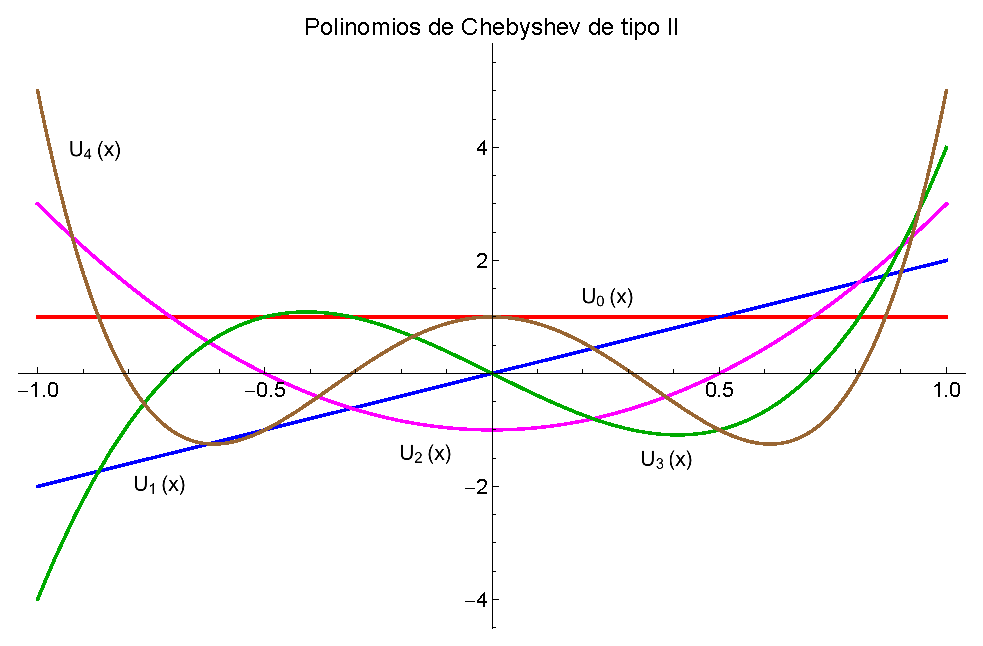
\includegraphics[scale=0.62]{Imagenes/Gram_Schmidt_Chebyshev_2.eps}
    \caption{Primeros polinomios de Chebyshev de orden $i = 0, 1, 2, 3, 4$ de tipo II.}
    \label{fig:figura_01}
\end{figure}

\section{Problemas Sturm-Liouville.}
\subsection{Interpretación física.}

Los sistemas Sturm-Liouville surgen típicamente de problemas de \textcolor{blue}{vibración} en la mecánica continua. En lenguaje físico, describen problemas de frontera correspondientes a ondas estacionarias simplemente armónicas.
\par
Comúnmente suponemos en física que cualquier movimiento ondulatorio se puede resolver en ondas estacionarias simplemente armónicas, cada una de las cuales oscila periódicamente con su frecuencia adecuada.
\par
Aunque los físicos comúnmente asumimos este resultado sobre la base de la evidencia experimental y la intuición,  en realidad se puede deducir rigurosamente de la teoría matemática del movimiento ondulatorio como un problema de frontera en las ecuaciones diferenciales.
\par
Veamos la interpretación física de las eigenfunciones de los sistemas de Sturm Liouville con tres ejemplos clásicos.

\subsection{Ecuación de onda.}

La EDP de una cuerda que vibra es:
\begin{align*}
\pdv[2]{y}{t} = c^{2} \, \pdv[2]{y}{x} \hspace{1.3cm} c^{2} = \dfrac{T}{\rho}
\end{align*}
Donde:
\begin{enumerate}[label=\roman*)]
\item $y$ es el desplazamiento lateral desde el punto de equilibrio.
\item $T$ es la tensión (constante)
\item $\rho$ la densidad de la cuerda (constante)
\end{enumerate}

Las ondas estacionarias simplemente armónicas se definen por la separación de variables:
\begin{align*}
y (x, t) = u (x) \, \cos k(t - t_{0})
\end{align*}

Para que la solución $y (x, t)$ satisfaga la ecuación de onda $y_{tt} = c^{2} \, y_{xx}$,  \emph{es necesario y suficiente} que:
\begin{align*}
\sderivada{u} + \lambda \, u = 0, \hspace{1.3cm} \lambda = \dfrac{k^{2}}{c^{2}}
\end{align*}
donde $k$ depende de la condición del extremo final.
\par
Para la cuerda que vibra,  \emph{es natural físicamente tener extremos fijos}, de modo que:
\begin{align*}
y (a, t) = y (b, t) = 0
\end{align*}
Esto hace que:
\begin{align*}
u (a) = u (b) = 0
\end{align*}

El eigenvalor perteneciente a cada eigenfunción \emph{es proporcional} a la frecuencia al cuadrado $k^{2}/4 \pi^{2}$.
\par
Esta relación, combinada con la analogía entre ondas mecánicas y electromagnéticas, ha llevado a los matemáticos a llamar al conjunto de eigenvalores como \textcolor{blue}{el espectro} de un sistema S-L.

\subsection{Vibraciones en una barra.}

Otra \emph{interpretación física} de los sistemas S-L la proporcionan \textcolor{blue}{las vibraciones longitudinales de una barra elástica} de rigidez local $p (x)$ y densidad $p (x)$.
\par
El desplazamiento longitudinal medio $v (x, t)$ de la sección de dicha barra desde su posición de equilibrio $x$ satisface la ecuación de onda:
\begin{align*}
\rho (x) \, \pdv[2]{v}{t} = \pdv{x} \bigg[ p (x) \, \pdv{v}{x} \bigg]
\end{align*}

Las oscilaciones armónicas simples (los \emph{modos normales} de oscilación) están dados por la separación de variables:
\begin{align*}
v (x, t) = u (x) \, \cos k(t - t_{0})
\end{align*}
Que son soluciones a la ecuación de S-L:
\begin{align*}
\dv{x} \bigg[ p (x) \, \dv{u}{x} \bigg] + k^{2} \, \rho (x) \, u = 0
\end{align*}
En este caso especial, $q = 0$ y $\lambda = k^{2}$.
\par
Para una barra finita, que se extiende en el intervalo $a \leq x \leq b$, se presentan naturalmente varias condiciones físicas de frontera:
\begin{enumerate}[label=\alph*)]
\item $u (a) = u (b) = 0$ extremos rígidamente fijos
\item $\pderivada{u} (a) = \pderivada{u} (b) = 0$ extremos libres
\item $\pderivada{u} (a) + \alpha u (a) = \pderivada{u} (b) + \beta u (b) = 0$ extremos sujetos elásticamente
\item $u (a) = u (b) \hspace{0.5cm} \pderivada{u} (a) = \pderivada{u} (b)$ restricciones periódicas
\end{enumerate}

Cada una de estas condiciones de punto final en $u$ \emph{implica una condición correspondiente} en $v (x, t)$, con $\dv*{x}$ reemplazada por $\pdv*{x}$.
\par
Las frecuencias naturales de vibración longitudinal (\textcolor{red}{tono musical fundamental} y \textcolor{blue}{sobretonos}) de una barra cuyos extremos se mantienen en cada una de las formas descritas son,  por lo tanto, las soluciones de los sistemas S-L y las condiciones apropiadas anteriores.

\subsection{Membrana oscilante.}

La EDP de una membrana oscilando es:
\begin{align*}
w_{tt} = c^{2} \, (w_{xx} + w_{yy}) = c^{2} \, (w_{rr} + r^{-1} \, w_{r} + r^{2} \, w_{\theta \theta})
\end{align*}
donde $r$, $\theta$ indican las coordenadas polares.
\par
Se puede encontrar una base de soluciones de onda estacionaria mediante la separación de variables:
\begin{align*}
w (r, \theta, t) = u (r) \, \left\{ \stackrel{\displaystyle \cos}{\sin} \right\} \, n \, \theta \, \cos \kappa (t - t_{0})
\end{align*}
Para que $w$ satisfaga la ecuación de membrana con $\kappa = c \, k$,  es \emph{necesario y suficiente} de que $u$ sea una solución de la ecuación de Bessel.
\par
La singularidad en $r = 0$ de la ecuación de Bessel está asociada con la singularidad en coordenadas polares en el origen.
\par
Si la membrana es un disco circular de radio $a$ (como el parche de un tambor),  las condiciones de frontera físicamente naturales son $u (a) = 0$ y $u(0)$ no singular.
\par
La última condición caracteriza las funciones de Bessel entre otras soluciones de la ecuación de Bessel, hasta un factor de normalización constante.
\end{document}